The goal was to perform real-time estimation of dynamically consistent joint kinematics and muscles activations, using a moving horizon estimation (MHE). 
In this example, a shoulder elevation motion is performed with a 4-DoFs arm actuated by 19 Hill-type muscle elements.
The control inputs of the model are the muscle activations.
The MHE implementation consists in splitting the OCP into a succession of smaller one for processing fixed-size subsets of the tracking data moving forward in time. 
Each time one subproblem is solved, a new measurement is acquired, the oldest one is discarded and a new subproblem is defined. 
Due to their similarities, the solution of the previous OCP is a good initial guess for the new one. 
The dynamic consistency of the final solution is enforced by continuity constraints on the initial state. 
Each objective function (Eq.~\ref{eq:ocp_exMHE}) was written as the sum of three terms: the first one corresponds to the tracking of reference joint angles, the second and third ones correspond to states and muscle activation regularization (i.e., least-square criteria): 

\[ 
\resizebox{0.9\columnwidth}{!}{$ 
\begin{aligned}
\mathcal{J} = &\int_t^{t+t_{mhe}}\underbrace{\omega_1´(\|q_{e} - q^*_{r}\|^{2})}_{\mathtt{TRACK\_STATE}}~ 
+ ~ \underbrace{\|q_{e}\|^2}_{\mathtt{MIN\_STATE}}
+ ~ \underbrace{\omega_2 \|u\|^2}_{\mathtt{MIN\_ACTIVATION}}~dt, 
\end{aligned}  
$}  
\addtag  
\label{eq:ocp_exMHE}  
\]  

\noindent where $\omega_1 =1e3$, $\omega_2 = 10$ and $t_{mhe}$ is duration of each sub-problem. $q_{e}$, $q^*_{r}$  and $u$ are respectively the reference and estimated joint angles, and muscles activations. 

In this example, reference data of an $8~s$ series of 4 arm elevations were generated at 100~Hz, by computer simulation, with co-activation on two antagonists muscles groups (triceps and biceps).
Using a windows size of 7 nodes, the estimator ran at about 50~Hz (one in two reference data frame was sent to the estimator to simulate experimental-like conditions), i.e., four times faster than standard biofeedback (13~Hz, \cite{kannape2013biofeedback}).
The estimator was able to forecast the movement kinematics (Fig.~\ref{fig:joints_angles_MHE}) with a consistent dynamics and a root mean square error of $0.02\pm6e\emph{-3}\text{~}^{\circ}$.
Due to co-contraction, the estimated muscles activations were lower than reference activations but with a similar pattern (Fig.~\ref{fig:muscles_excitations_MHE}).  
For a more in-depth analysis of the real-time capabilities of \textit{bioptim}, see \cite{bailly2020real}.
 

\begin{figure*}[t!] 
\centering 
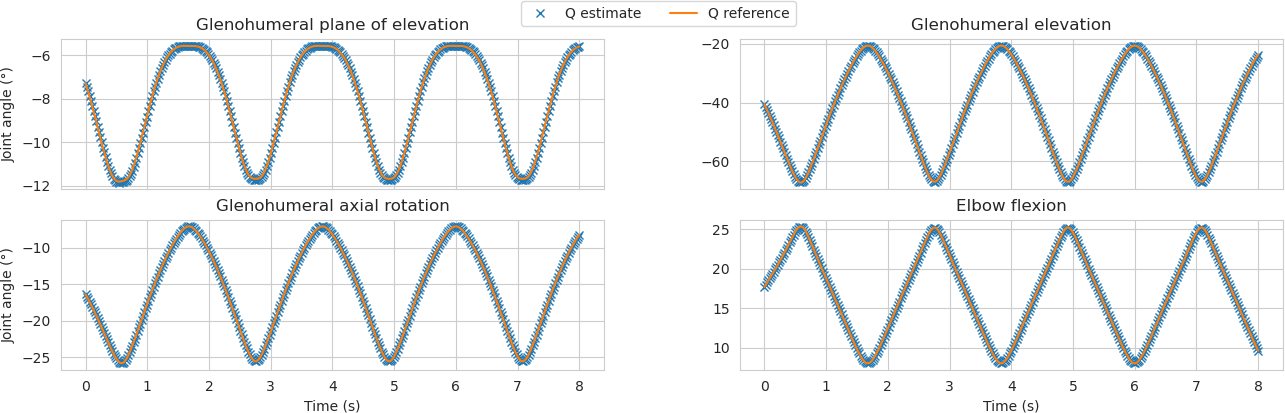
\includegraphics[width=\textwidth]{figures/Articular_angle_MHE.png}\\ 
\caption{Time histories of estimate joints angles (blue cross) and reference joints angles (orange line).} 
\label{fig:joints_angles_MHE} 
\end{figure*} 

\begin{figure*}[t!] 
\centering 
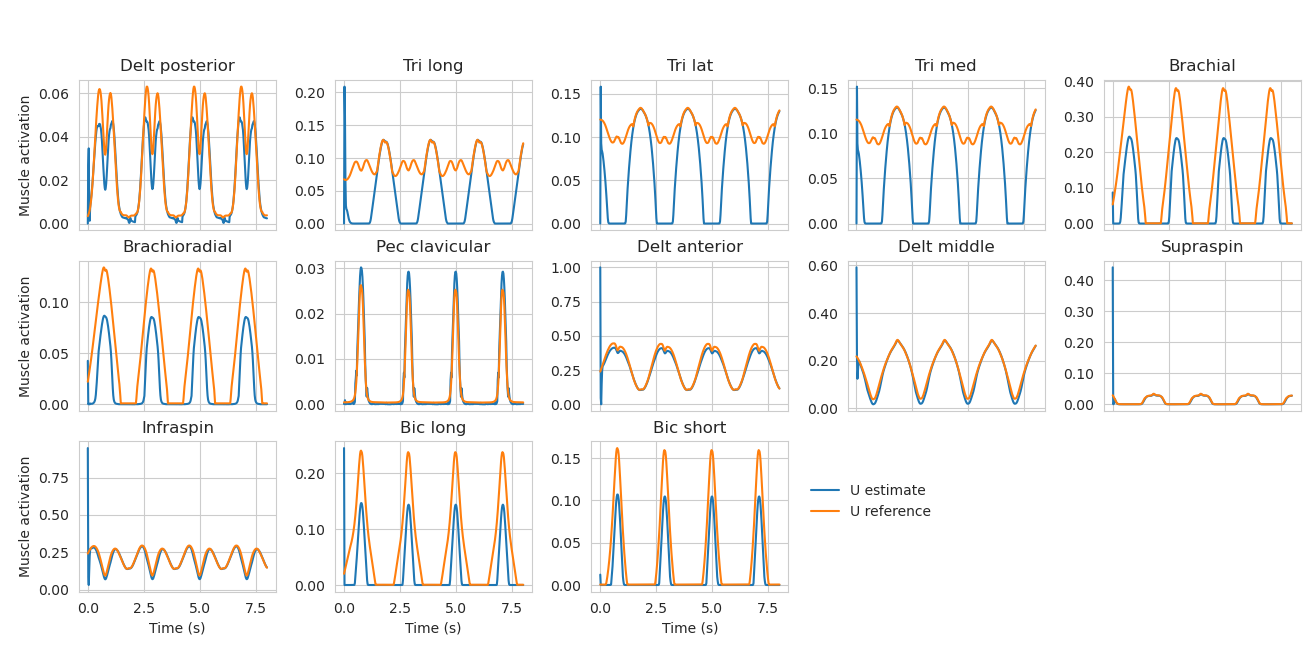
\includegraphics[width=\textwidth]{figures/Muscles_excitations_MHE.png}\\ 
\caption{Time histories of estimate muscles activations (blue) and co-contracted muscles activations (orange) with significative action on motion (peaks activation level $>$ 0.1). 
Muscles' abbreviations stand for (from left to right and top to bottom): Triceps long head, lateral and medial, Brachial, Brachioradialis, Deltoid Anterior and Middle, Infraspinatus, Subscapularis, Biceps Brachial long and short head.} 
\label{fig:muscles_excitations_MHE} 
\end{figure*} 

